\documentclass{beamer}
\usetheme{Madrid}
\usecolortheme{whale}
\usepackage{booktabs} 
\usepackage{listings}
\usepackage{amsmath}
\usepackage{graphicx}
\usepackage{tikz}
\usepackage{algorithm}
\usepackage{algpseudocode}
\usepackage{subfigure}
\usepackage{subcaption}

\title{Analysis of CVAE Implementation}
\subtitle{Coulomb Explosion Atomic Reconstruction}
\author{A.Ghanaatian\and Supervisor: Prof. Caragea}
\date{\today}

\begin{document}

\begin{frame}
    \titlepage
\end{frame}

\section{Data Analysis}

\begin{frame}{Dataset Overview}
    \begin{itemize}
        \item \textbf{Input Features} (Position Coordinates):
        \begin{itemize}
            \item Carbon (cx, cy, cz)
            \item Oxygen (ox, oy, oz)
            \item Sulfur (sx, sy, sz)
        \end{itemize}
        \item \textbf{Target Features} (Momenta):
        \begin{itemize}
            \item Carbon (pcx, pcy, pcz)
            \item Oxygen (pox, poy, poz)
            \item Sulfur (psx, psy, psz)
        \end{itemize}
        \item \textbf{Goal:} Solving inverse problem
    \end{itemize}
\end{frame}

\begin{frame}{Data Preprocessing}
    \begin{columns}
        \column{0.5\textwidth}
        \textbf{Data Split}
        \begin{itemize}
            \item Training: 70\% (Primary training)
            \item Validation: 15\% (Checking overfitting)
            \item Test: 15\% (Final evaluation)
        \end{itemize}
        
        \column{0.5\textwidth}
        \textbf{Normalization}
        \begin{itemize}
            \item Position: StandardScaler
            \item It has inverse function
            \item Momenta: None!
        \end{itemize}
    \end{columns}
\end{frame}

\section{Model Architecture}

\begin{frame}{CVAE Architecture Overview}
    \begin{itemize}
        \item \textbf{Encoder Network}:
        \begin{itemize}
            \item Input dimension: 9
            \item Hidden layers: [256, 512, 1024]
            \item Output: $\mu$ and $\log\sigma$ vectors (1024 each)
        \end{itemize}
        \item \textbf{Latent Space}:
        \begin{itemize}
            \item Dimension: 1024
            \item Reparameterization trick
            \item Gaussian prior (N(0,1))
        \end{itemize}
        \item \textbf{Decoder Network}:
        \begin{itemize}
            \item Input: Concatenated [z, condition]
            \item Hidden layers: [512, 256]
            \item Output dimension: 9
        \end{itemize}
    \end{itemize}
\end{frame}

\begin{frame}{Detailed Layer Configuration}
    \begin{itemize}
        \item \textbf{Layer Sizes}:
        \begin{align*}
            \text{Input} &\rightarrow 9 \\
            \text{Encoder}_1 &\rightarrow 256 \\
            \text{Encoder}_2 &\rightarrow 512 \\
            \text{Encoder}_3 &\rightarrow 1024 \\
            \text{Latent} &\rightarrow 1024 \\
            \text{Decoder}_1 &\rightarrow 512 \\
            \text{Decoder}_2 &\rightarrow 256 \\
            \text{Output} &\rightarrow 9
        \end{align*}
        \item \textbf{Activation}: Sigmoid
        \item \textbf{Parameter Sharing}: None between encoder and decoder
    \end{itemize}
\end{frame}


\section{Training Configuration}


\begin{frame}{Model Architecture}
    \centering
    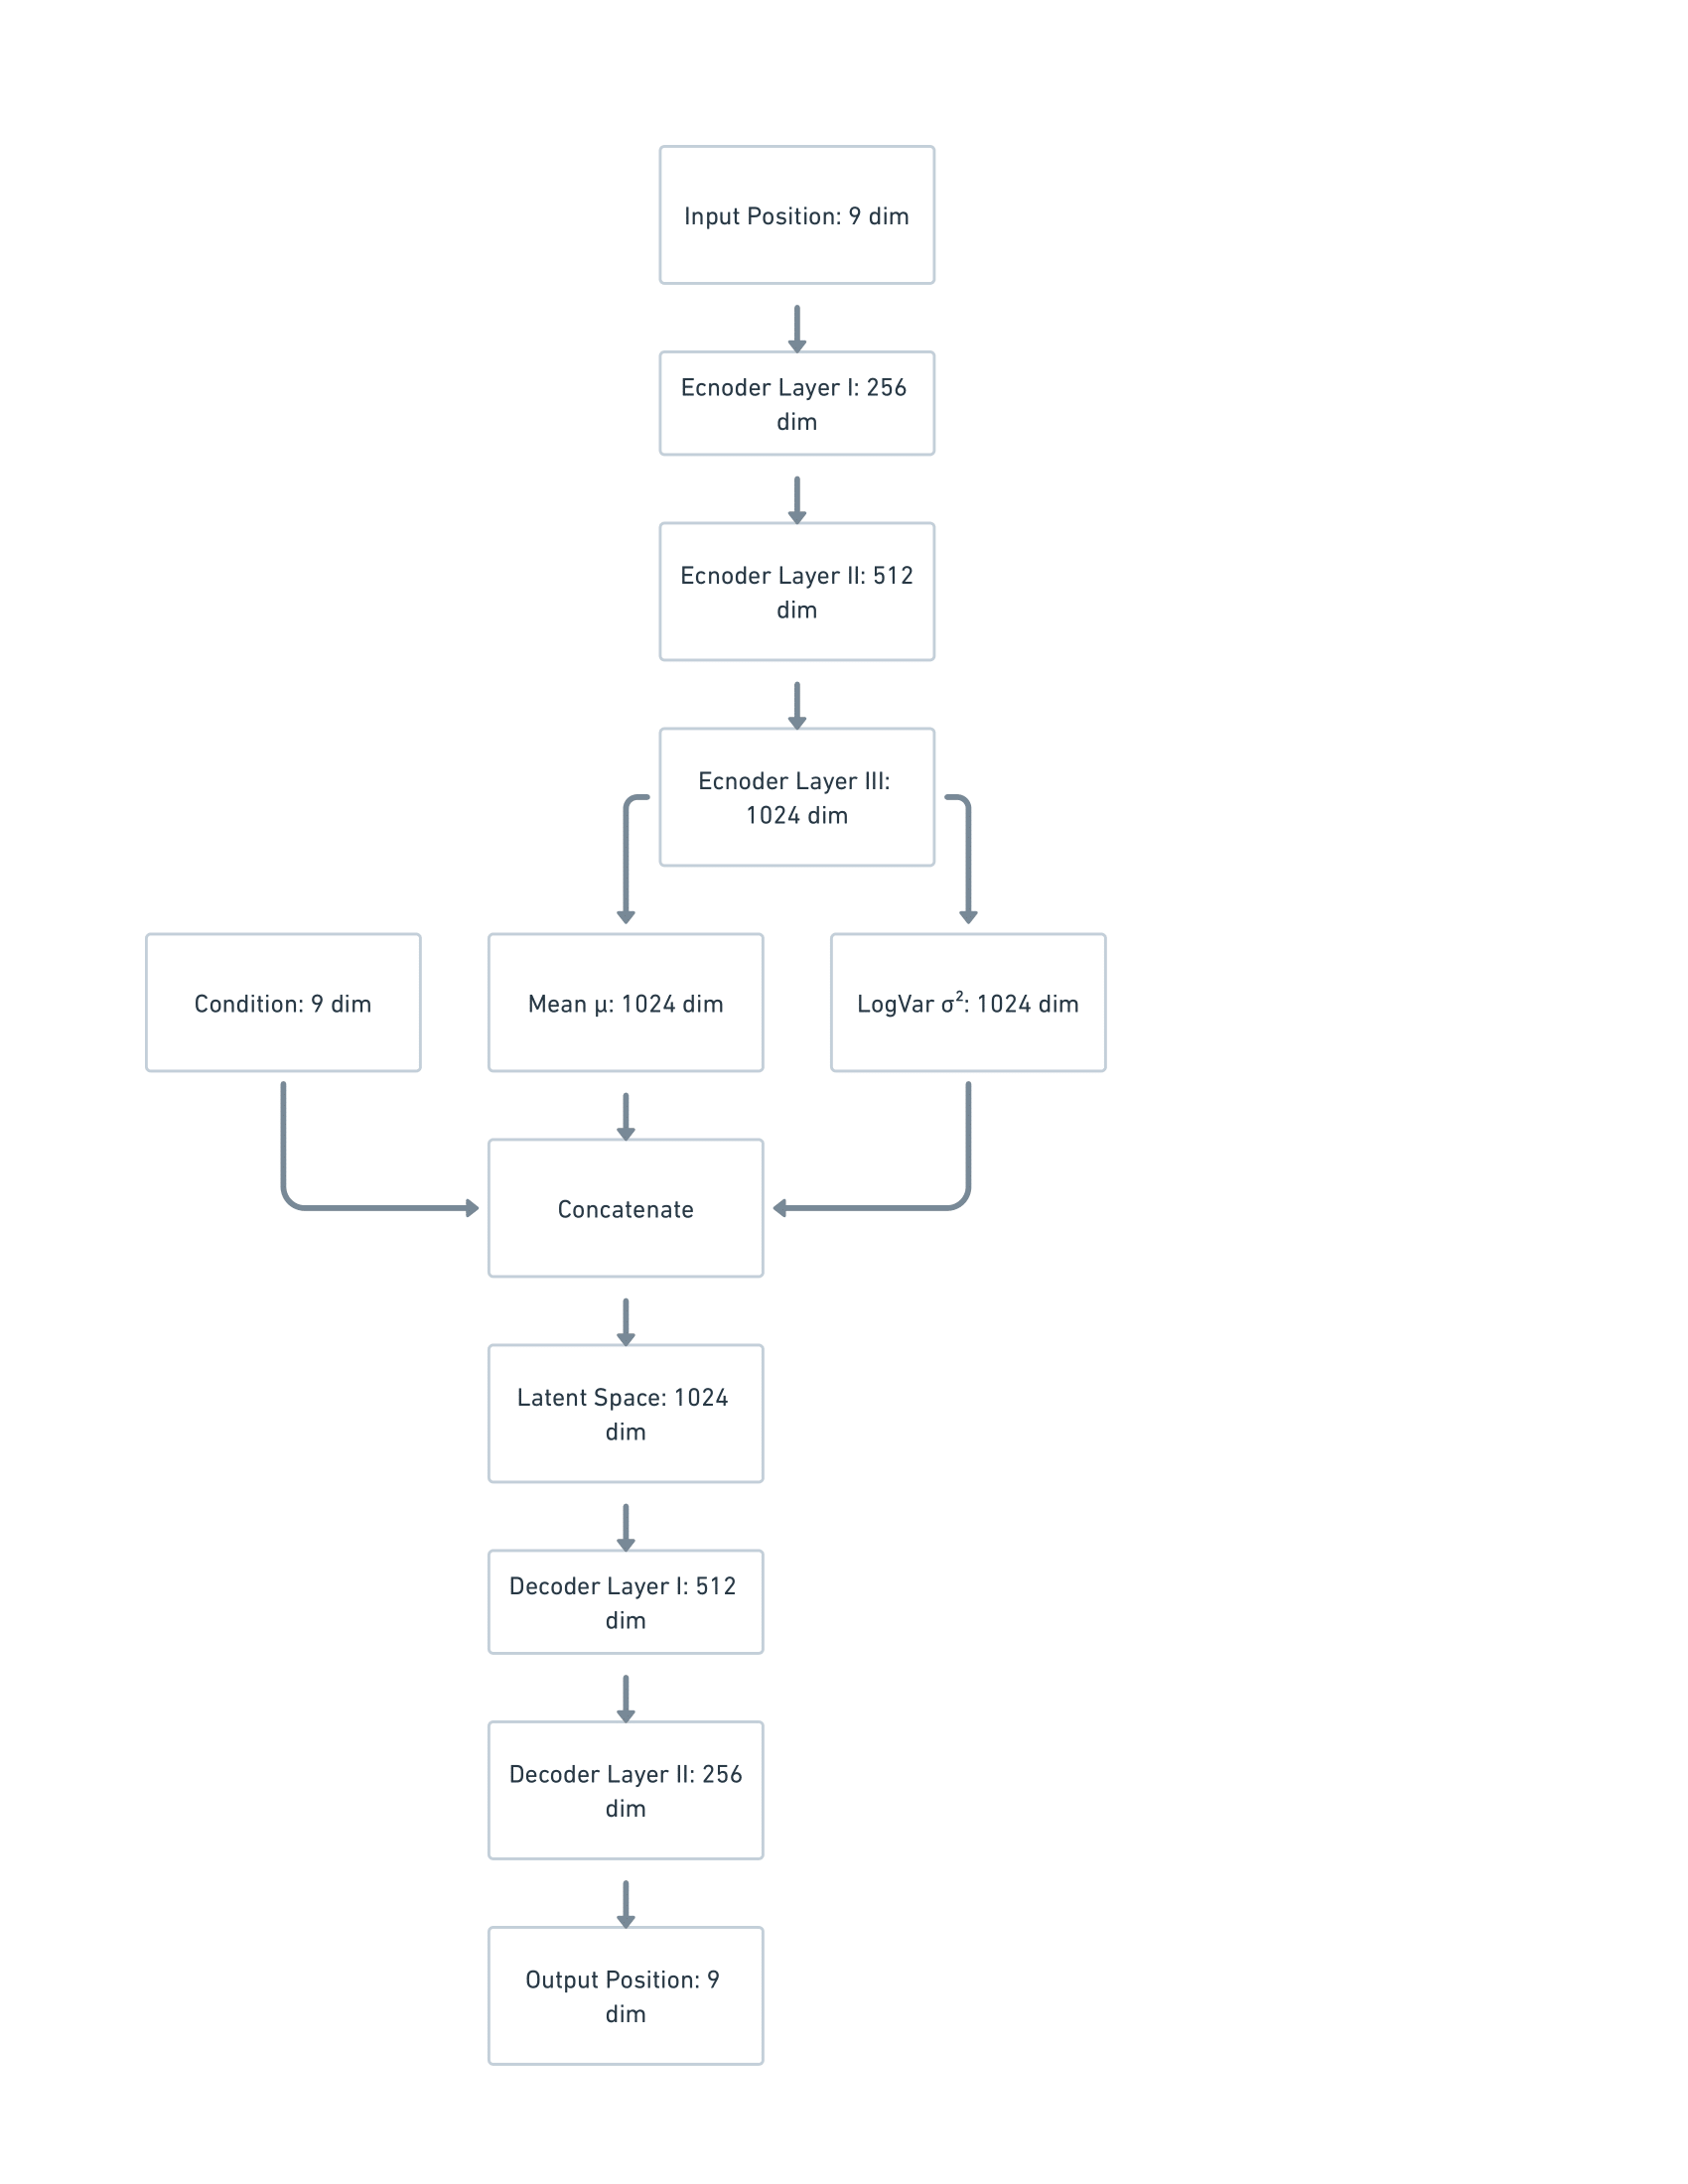
\includegraphics[height=0.9\textheight]{ma.png}
\end{frame}


\begin{frame}{Hyperparameters}
    \begin{columns}
        \column{0.5\textwidth}
        \textbf{Basic Parameters}
        \begin{itemize}
            \item Epochs: 200
            \item Batch Size: 256
            \item Learning Rate: $1 \cdot 10^{-4}$
            \item Encoders Layer Size: [256, 512, 1024]
            \item Decoders Layer Size: [512, 256]
            \item Number of Hidden Layers: 3
        \end{itemize}
        
        \column{0.5\textwidth}
        \textbf{Advanced Parameters}
        \begin{itemize}
            \item Latent Dimension: 1024
            \item Early Stopping Patience: 100
            \item Minimum Delta: $1 \cdot 10^{-5}$
            \item L1 Lambda: $False$
            \item L2 Lambda: $1 \cdot 10^{-2}$
            \item Gradient Clip: 5.0
        \end{itemize}
    \end{columns}
\end{frame}

\begin{frame}{Loss Function Components}
    \begin{align*}
        \mathcal{L}_{\text{total}} &= \mathcal{L}_{\text{recon}} + \mathcal{L}_{\text{KL}} + \lambda\mathcal{L}_{\text{L1}} \\[1em]
        \mathcal{L}_{\text{recon}} &= \text{MSE}(x_{\text{recon}}, x) \\[0.5em]
        \mathcal{L}_{\text{KL}} &= -\frac{1}{2N}\sum(1 + \log\sigma^2 - \mu^2 - \sigma^2) \\[0.5em]
        \mathcal{L}_{\text{L1}} &= \sum|\theta|
    \end{align*}
    where:
    \begin{itemize}
        \item $x_{\text{recon}}$ is the reconstructed output
        \item $\mu, \sigma$ are latent space parameters
        \item $\theta$ represents model parameters
        \item $\lambda = 1.41 \cdot 10^{-4}$ (L1 regularization strength)
    \end{itemize}
\end{frame}

\section{Regularization Techniques}

\begin{frame}{L2 Regularization Deep Dive}
\textbf{Mathematical Formulation:}
$L_{\text{reg}}(\theta) = L(\theta) + \lambda \sum_{i=1}^{n} \theta_i^2 $
\begin{itemize}
    \item \textbf{Properties}:
    \begin{itemize}
        \item Creates circular/spherical constraint region
        \item Assumes Gaussian prior on weights
        \item Differentiable everywhere
    \end{itemize}
    \item \textbf{Mathematical Characteristics}:
    \begin{itemize}
        \item Gradient proportional to parameter value
        \item Strictly convex optimization
        \item Handles multicollinearity effectively
    \end{itemize}
    \item \textbf{Effects}:
    \begin{itemize}
        \item Shrinks weights proportionally
        \item Distributes importance across correlated features
        \item Produces unique solutions
    \end{itemize}
\end{itemize}
\end{frame}

\begin{frame}{Additional Regularization Techniques}
    \begin{itemize}
        \item \textbf{Early Stopping}:
        \begin{itemize}
            \item Monitors validation loss
            \item Patience: 100 epochs
            \item Minimum improvement: $1 \cdot 10^{-5}$
        \end{itemize}
        \item \textbf{Gradient Clipping}:
        \begin{itemize}
            \item Maximum norm: 5.0
            \item Prevents exploding gradients
            \item Stabilizes training
        \end{itemize}
        \item \textbf{Data Normalization}:
        \begin{itemize}
            \item StandardScaler for Positions
            \item No Normalization for Momanta
            \item Prevents scaling issues
            \item Consider inverting to original scale for Evaluation
        \end{itemize}
    \end{itemize}
\end{frame}

\section{Training Process}

\begin{frame}{Training Algorithm}
    \begin{algorithm}[H]
    \caption{CVAE Training Process}
    \begin{algorithmic}[1]
        \For{epoch in range(EPOCHS)}
            \For{batch in train\_loader}
                \State $x, \text{condition} \gets \text{batch}$
                \State $\mu, \log\sigma \gets \text{encoder}(x)$
                \State $z \gets \mu + \epsilon * \exp(0.5 * \log\sigma)$
                \State $x_{\text{recon}} \gets \text{decoder}(z, \text{condition})$
                \State Compute loss $\mathcal{L}_{\text{total}}$
                \State Backward pass and update weights
                \State Clip gradients at 5.0
            \EndFor
            \State Validate and check early stopping
        \EndFor
    \end{algorithmic}
    \end{algorithm}
\end{frame}

\begin{frame}{Training Monitoring}
    \begin{itemize}
        \item \textbf{Loss Tracking}:
        \begin{itemize}
            \item Training loss per epoch
            \item Validation loss per epoch
            \item Individual loss components
        \end{itemize}
        \item \textbf{Model Checkpointing}:
        \begin{itemize}
            \item Save best model state
            \item Based on validation loss
            \item Restore for testing
        \end{itemize}
        \item \textbf{Early Stopping Logic}:
        \begin{itemize}
            \item Monitor validation loss
            \item Reset counter on improvement
            \item Stop when patience exceeded
        \end{itemize}
    \end{itemize}
\end{frame}

\section{Evaluation}

\begin{frame}{Evaluation Metrics}
    \begin{itemize}
        \item \textbf{Mean Relative Error (MRE)}:
        \[ \text{MRE} = \frac{1}{n}\sum_{i=1}^{n}\frac{|y_{\text{pred},i} - y_{\text{true},i}|}{|y_{\text{true},i}| + \epsilon} \]
        \item \textbf{Latent Space Statistics}:
        \begin{itemize}
            \item Best Test MRE: $48\%$
        \end{itemize}
    \end{itemize}
\end{frame}

\begin{frame}{Other Metrics}
    \begin{table}
        \centering
        \begin{tabular}{lcc}
            \toprule
            \textbf{Dataset} & \textbf{MRE} & \textbf{MSE} \\
            \midrule
            Training & 0.553 & 5.128 \\
            Validation & 0.489 & 5.152 \\
            Test & 0.486 & 5.263 \\
            \bottomrule
        \end{tabular}
        \caption{Model Performance Metrics}
        \label{tab:metrics}
        \footnotesize{MRE: Mean Relative Error, MSE: Mean Squared Error}
    \end{table}
\end{frame}

\begin{frame}{Learning Curve Plot}
    \begin{columns}[c] % 'c' for center alignment vertically
        \column{1.05\textwidth}  % slightly reduced from 0.5 to allow spacing
            \centering
            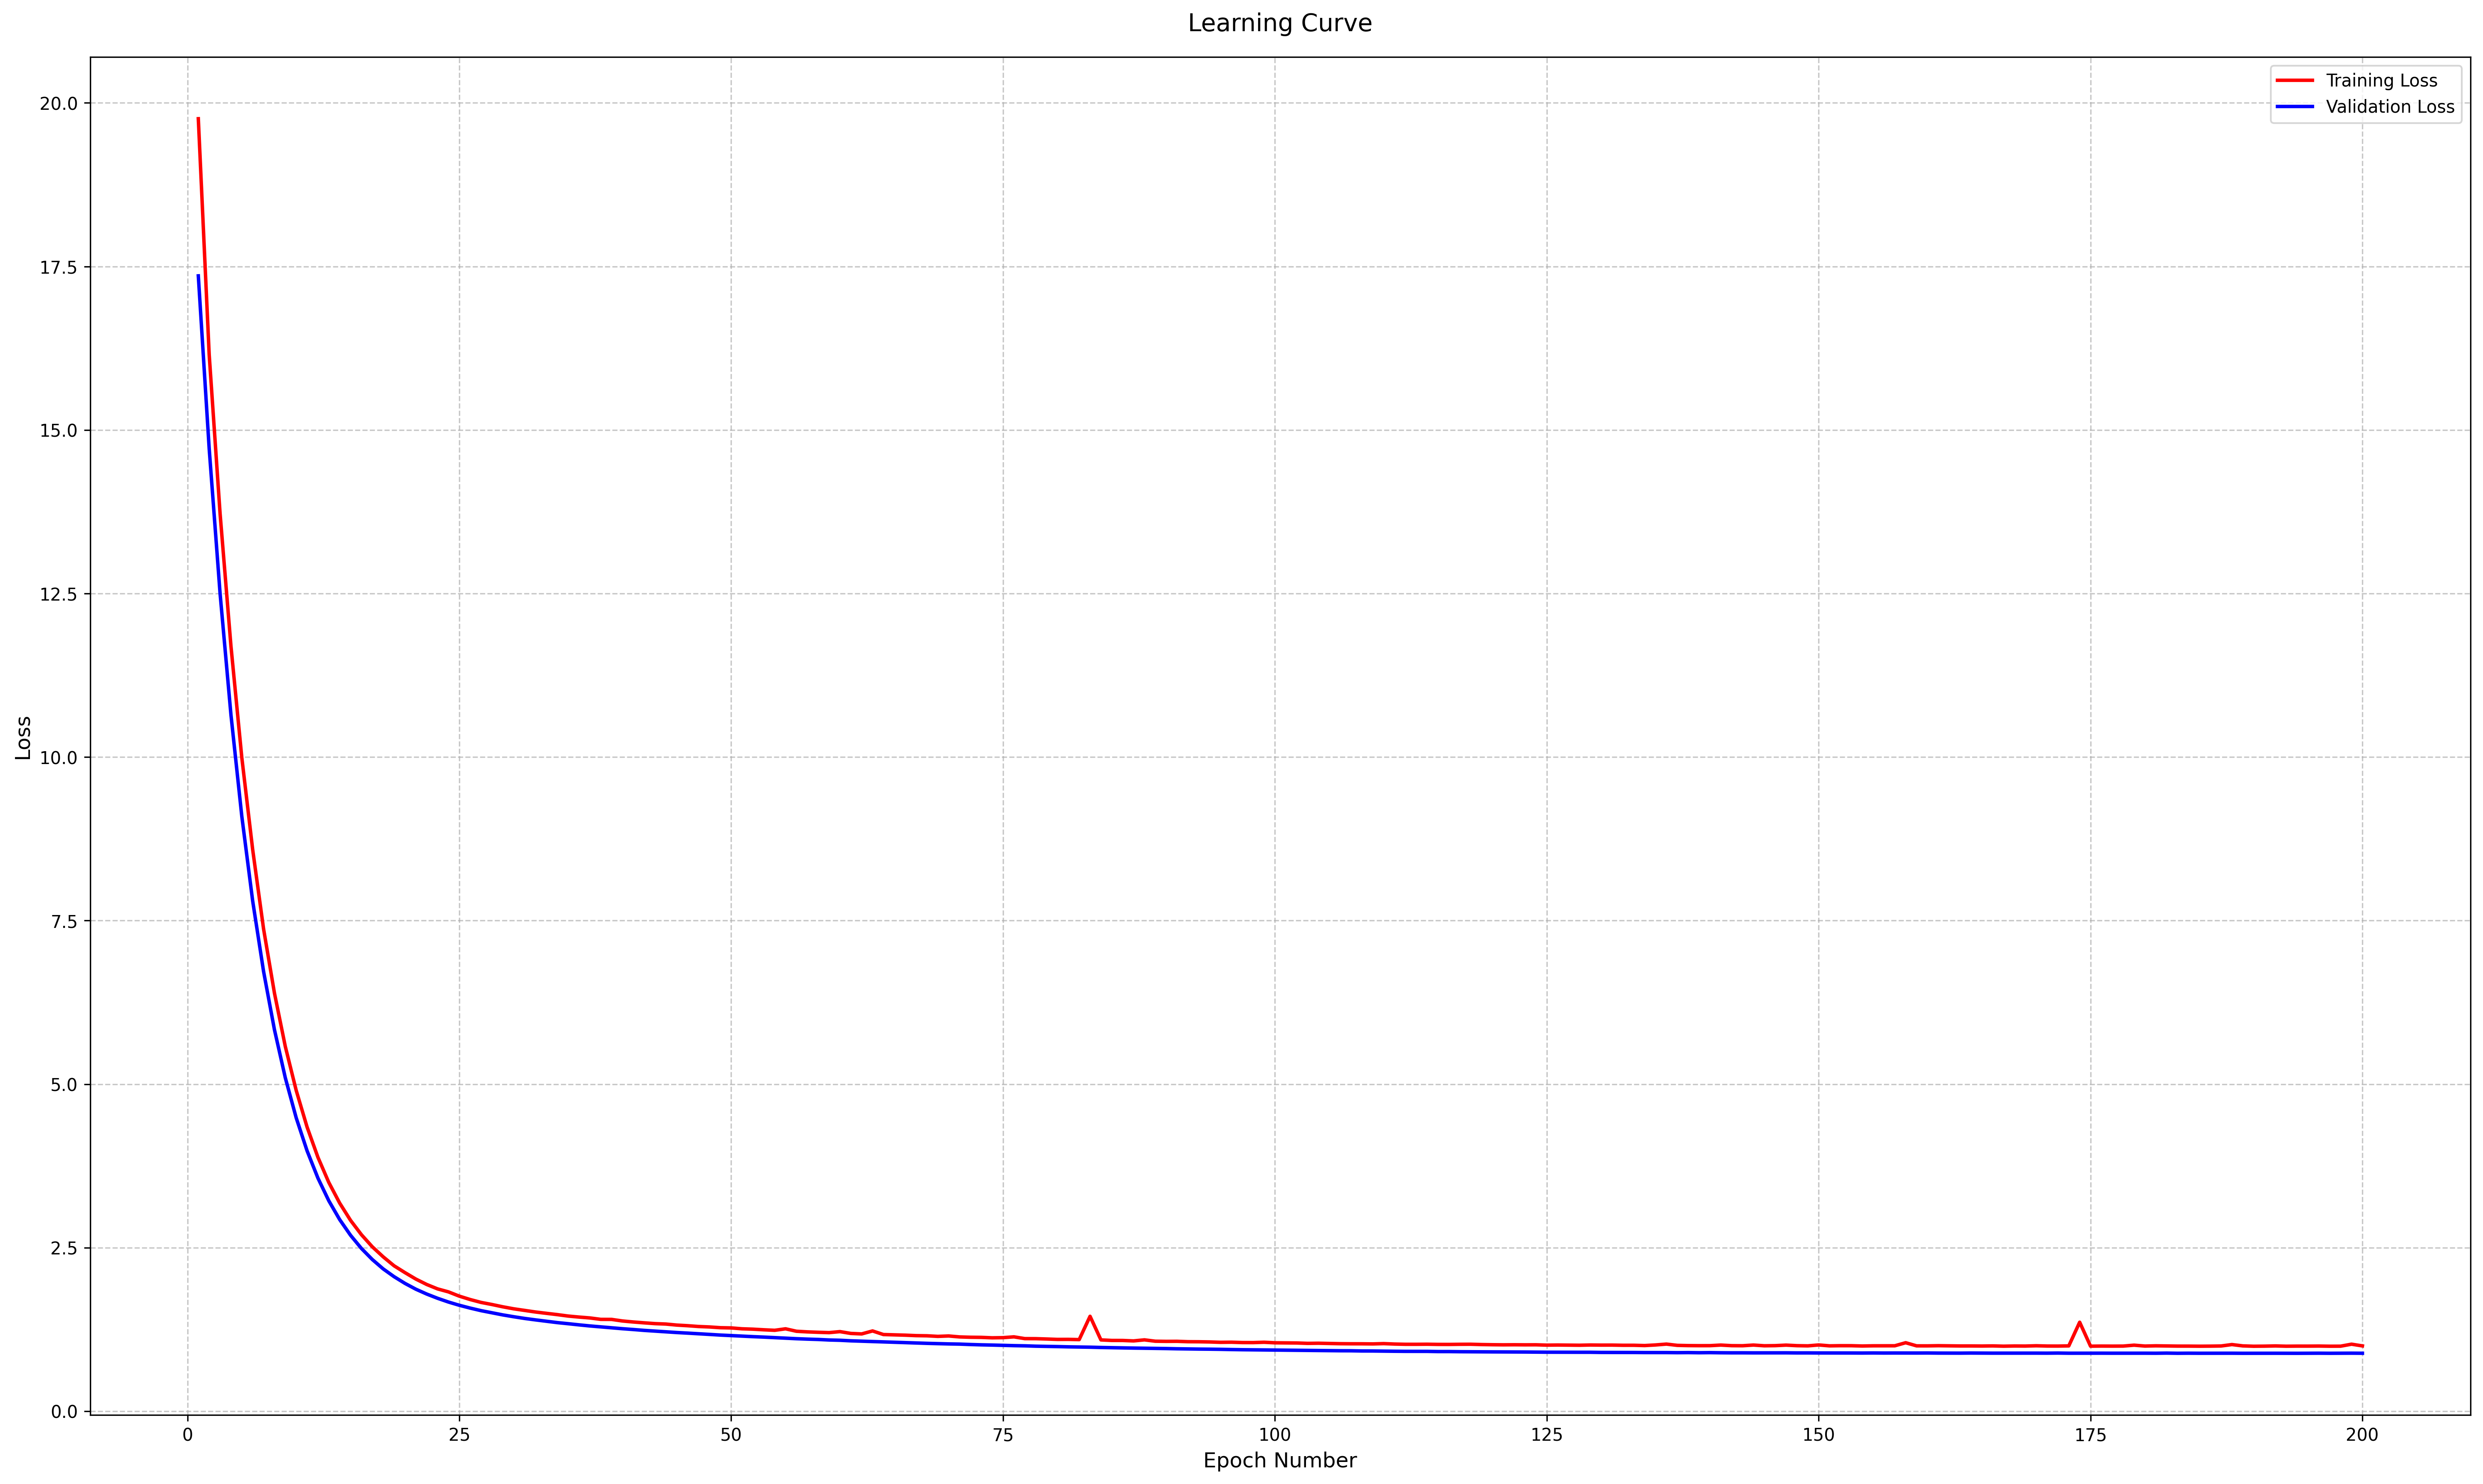
\includegraphics[width=\linewidth]{first.png}
            \text{}  % Using text instead of caption
        
    \end{columns}
\end{frame}


\end{document}